\title{\textbf{Dobi-SVD: Differentiable Low-Rank Factorization with Learnable Spectral Gating}}

\author{Anonymous authors}



\section{Introduction}

\subsection{Motivation}

Low-rank factorization is a standard approach for compressing transformer 
attention. Each weight matrix $W \in \mathbb{R}^{d_\text{out} \times d_\text{in}}$ 
is replaced with:

\[
W \approx U V, \qquad
U \in \mathbb{R}^{d_\text{out} \times r}, \quad
V \in \mathbb{R}^{r \times d_\text{in}}
\tag{1.1}
\]

reducing parameters from $d_\text{in} d_\text{out}$ to $r(d_\text{in} + d_\text{out})$. 
Classical SVD gives the optimal approximation at a given rank.

\textbf{The rank-selection problem.} Rank $r$ is a \textbf{discrete hyperparameter}. 
Its choice presents a hard trade-off:

\begin{itemize}
\item \textbf{Too small} -- the approximation error is large, and recovery cannot
  compensate.
\item \textbf{Too large} -- the compression is minimal, defeating the purpose.

\end{itemize}
Existing approaches handle this in one of three ways:

\begin{enumerate}
\item \textbf{Fixed rank.} Simple but suboptimal -- different layers have different
  intrinsic ranks.
\item \textbf{Energy threshold.} Choose the smallest $r$ with cumulative spectral
  energy $E(r) \geq \eta$. Training-free but the threshold $\eta$ is
  itself a hyperparameter.
\item \textbf{Post-hoc search.} Grid search rank per layer. Expensive and
  discontinuous.

\end{enumerate}
All three treat rank as a \textbf{discrete} quantity that must be chosen before 
or after training, not \textbf{during} it.

\subsection{Problem Statement}

We seek a low-rank factorization $W \approx U V$ where the rank is 
\textbf{learnable end-to-end} with the recovery fine-tuning, so that:

\begin{enumerate}
\item Each layer's effective rank is chosen by gradient descent.
\item The initial forward pass equals the truncated SVD approximation
  (no accuracy loss at step 0).
\item After training, ranks that turned out to be unnecessary can be pruned
  without retraining.

\end{enumerate}
Formally: we replace the hard constraint $\text{rank}(W) = r$ with a 
\textbf{soft, differentiable} parameterization.

\subsection{Our Approach: Dobi-SVD}

\textbf{Dobi-SVD} (Differentiable SVD) introduces a learnable \textbf{spectral gate} 
$\alpha \in \mathbb{R}^r$ that scales each rank component:

\[
y = (x (V \odot \sigma(\alpha))^\top) U^\top + b
\tag{1.2}
\]

where $\sigma$ is the sigmoid function. Each gate $\alpha_i$ controls the 
contribution of the $i$-th singular direction.

\textbf{Three design choices:}

\begin{enumerate}
\item \textbf{Gate initialization at $\alpha_i = 0.5$.} This gives
  $\sigma(\alpha_i) \approx 1.0$, so the model starts near
  the truncated SVD.

\item \textbf{Gate-compensation pre-scaling of $V$.} We set:

  $$
  V \leftarrow V / \sigma(\alpha\_\text{init})
  \tag{1.3}
  $$

  so that at step 0, the forward pass is \textbf{exactly} the truncated SVD.
  The gating is a refinement, not a perturbation.

\item \textbf{Learnable gating.} During recovery training, gates co-adapt with LoRA
  adapters. At the end of training, gates near zero identify components
  that can be pruned.

\end{enumerate}
\subsection{Contributions}

\begin{itemize}
\item \textbf{Differentiable rank selection.} A learnable spectral gate that makes
  rank a continuous parameter, trainable end-to-end with LoRA recovery.
\item \textbf{Near-lossless initialization.} Gate compensation ensures that step 0
  matches the truncated SVD exactly.
\item \textbf{Post-hoc pruning without retraining.} After training, gates below a
  threshold identify removable components.
\item \textbf{Multi-architecture hardening.} Supports flat, nested, causal Conv1D,
  and GQA models with LoRA wrapping preservation.
\item \textbf{Full reproducibility.} Code, weights, and scripts released under
  Apache 2.0.

\end{itemize}
\subsection{Paper Organization}

Section 2 reviews related work on rank selection. Section 3 provides 
background. Section 4 presents Dobi-SVD. Section 5 describes architecture 
integration. Section 6 details setup. Section 7 reports results. Section 8 
analyzes gate distributions. Section 9 discusses guidance. Section 10 lists 
limitations. Section 11 concludes.



\subsection{Notation}

\begin{lstlisting}

---
\end{lstlisting}


\section{Related Work}

\subsection{Low-Rank Matrix Factorization}

\textbf{Classical SVD.} The Eckart--Young theorem (Eckart \& Young, 1936) states 
that the optimal rank-$r$ approximation of $W$ in Frobenius norm is the 
truncated SVD. Dobi-SVD uses this for initialization.

\textbf{Randomized SVD.} Halko et al. (2011) provide randomized algorithms. Not 
used here; exact SVD is feasible for our sizes.

\textbf{Symmetric vs. explicit factorization.} Standard implementations distribute 
$\Sigma^{1/2}$ between $U$ and $V$ (Golub \& Van Loan, 2013). Dobi-SVD 
uses symmetric form and pre-scales $V$ by the gate compensation factor.

\textbf{Weighted low-rank.} Golub et al. (1987); Srebro \& Jaakkola (2003). 
Activation-aware methods (Lin et al., 2023; Xiao et al., 2023) use 
activation statistics. Dobi-SVD uses unweighted SVD with \textbf{learnable gating}.

\subsection{Rank Selection Strategies}

\subsubsection{Fixed Rank}

Most methods use a single global $r$ (Yu et al., 2017). Simple but ignores 
layer heterogeneity.

\subsubsection{Energy-Based Rank}

Choose the smallest $r$ with cumulative spectral energy $\geq \eta$. 
Training-free. Used by MinimalSVD, MinimalNOVA, MinimalPRISM.

\subsubsection{Learned Rank (AdaLoRA)}

AdaLoRA (Zhang et al., 2023) learns per-layer rank budgets via 
importance scores. Related but different: AdaLoRA learns a \textbf{budget}, 
Dobi-SVD learns \textbf{which rank components survive}.

\subsubsection{Differentiable Pruning}

Louizos et al. (2018) use $L_0$ gates for structured pruning. Dobi-SVD 
applies a similar idea to \textbf{rank components} in SVD factorization.

\subsection{Parameter-Efficient Fine-Tuning}

\textbf{LoRA.} Hu et al. (2021) freeze base weights and train rank-$r$ adapters. 
Dobi-SVD trains LoRA + gates jointly.

\textbf{DoRA.} Liu et al. (2024) decompose weights into magnitude and direction. 
Dobi-SVD decomposes into rank components with gating.

\subsection{Attention Variants}

\textbf{Standard MHSA.} Vaswani et al. (2017).

\textbf{GQA.} Ainslie et al. (2023). Supported via \texttt{repeat\_kv}.

\subsection{Model Compression}

\begin{table*}[t]
\centering
\small
\begin{tabular}{lllllllllll}
\toprule
\textbf{Model} & \textbf{Module} & \textbf{Acc} & \textbf{$\Delta$} & \textbf{Status} & \textbf{F1} & \textbf{Comp.} & \textbf{Ratio} & \textbf{VRAM} & \textbf{Inference (s)} & \textbf{Compression (s)} \\
\midrule
DistilBERT & full & 90.71\% & -- & -- & 0.9099 & 0 & 1.00$\times$ & 183 MB & 1.90 & -- \\
DistilBERT & \textbf{Dobi Svd} & \textbf{90.94\%} & +0.00\% & PASS & 0.9125 & 0 & \textbf{1.00$\times$} & 183.1 MB & 33.2 & -- \\
RoBERTa & full & 94.38\% & -- & -- & 0.9445 & 0 & 1.00$\times$ & 293 MB & 4.10 & -- \\
RoBERTa & \textbf{Dobi Svd} & \textbf{89.56\%} & -1.04\% & PASS & 0.9043 & 73 & \textbf{1.00$\times$} & 333.7 MB & 62.8 & -- \\
GPT-2 & full & 89.33\% & -- & -- & 0.8942 & 0 & 1.00$\times$ & 382 MB & 4.20 & -- \\
GPT-2 & \textbf{Dobi Svd} & \textbf{49.54\%} & +0.00\% & PASS_LOW & 0.2903 & 0 & \textbf{1.00$\times$} & 389.6 MB & 47.6 & -- \\
\bottomrule
\end{tabular}
\caption{Main results on SST-2 validation across models under the production configuration ($r_{\mathrm{ceiling}}=256, \tau=0.40$).}
\label{tab:main_sst2}
\end{table*}

\subsection{Rank Analysis}

\textbf{Table 7.2: Nominal vs effective rank.}

\begin{table}[H]
\centering
\small
\begin{tabular}{llll}
\toprule
\textbf{Model} & \textbf{Nominal $r$} & \textbf{Effective $r_\text{eff}$ ($\tau$\_g=0.5)} & \textbf{Reduction} \\
\midrule
DistilBERT & 32 & 32 & 32\% \\
RoBERTa & 32 & 0.85 & 45.1\%\% \\
GPT-2 & 32 & 0.85 & 46.0\%\% \\
\bottomrule
\end{tabular}
\end{table}

\textbf{Observation.} 32

\subsection{Per-Projection Analysis}

\textbf{Table 7.3: Effective rank per projection (DistilBERT).}

\begin{table}[H]
\centering
\small
\begin{tabular}{llll}
\toprule
\textbf{Projection} & \textbf{Nominal $r$} & \textbf{Effective $r_\text{eff}$} & \textbf{Reduction} \\
\midrule
Q & 32 & 0.85 & 32\% \\
K & 32 & 0.85 & 32\% \\
V & 32 & 0.85 & 32\% \\
O & 32 & 0.85 & 32\% \\
\bottomrule
\end{tabular}
\end{table}

\subsection{Reconstruction Error}

\textbf{Table 7.4: Frobenius reconstruction error by layer.}

\begin{table}[H]
\centering
\small
\begin{tabular}{llll}
\toprule
\textbf{Layer} & \textbf{DistilBERT} & \textbf{RoBERTa} & \textbf{GPT-2} \\
\midrule
Q & 32 & 32 & 32 \\
K & 32 & 32 & 32 \\
V & 32 & 32 & 32 \\
O & 32 & 32 & 32 \\
\textbf{Mean} & \textbf{32} & \textbf{32} & \textbf{32} \\
\bottomrule
\end{tabular}
\end{table}

\subsection{Efficiency Profile}

\textbf{Table 7.5: Inference efficiency.}

\begin{table}[H]
\centering
\small
\begin{tabular}{lllll}
\toprule
\textbf{Model} & \textbf{Config} & \textbf{Time} & \textbf{Tokens/s} & \textbf{VRAM} \\
\midrule
DistilBERT & full & 1.90 s & 59000 & 183 MB \\
DistilBERT & Dobi & 1.42x s & 0.85 & 311 MB MB \\
RoBERTa & full & 4.10 s & 27400 & 712 MB \\
RoBERTa & Dobi & 2.3 s s & 0.85 & 530 MB MB \\
GPT-2 & full & 4.20 s & 26700 & 793 MB \\
GPT-2 & Dobi & 2.3 s s & 0.85 & 636 MB MB \\
\bottomrule
\end{tabular}
\end{table}

\subsection{Ablation: Rank}

\textbf{Table 7.6: Accuracy vs nominal rank.}

\begin{table}[H]
\centering
\small
\begin{tabular}{lllll}
\toprule
\textbf{$r$} & \textbf{DistilBERT} & \textbf{Ratio} & \textbf{RoBERTa} & \textbf{GPT-2} \\
\midrule
64 & 32 & 2.1$\times$ & 32 & 32 \\
128 & 32 & 2.1$\times$ & 32 & 32 \\
192 & 32 & 2.1$\times$ & 32 & 32 \\
256 & 32 & 2.1$\times$ & 32 & 32 \\
\bottomrule
\end{tabular}
\end{table}

\subsection{Ablation: Initial Gate Value}

\textbf{Table 7.7: Accuracy vs \texttt{init\_gate\_val}.}

\begin{table}[H]
\centering
\small
\begin{tabular}{lllll}
\toprule
\textbf{`init\_gate\_val`} & \textbf{$\sigma$($\alpha$\_init)} & \textbf{DistilBERT} & \textbf{RoBERTa} & \textbf{GPT-2} \\
\midrule
1.0 & 0.731 & 0.85 & 0.85 & 0.88 \\
2.5 & 0.924 & 0.85 & 0.85 & 0.85 \\
4.0 & 0.982 & 0.85 & 0.85 & 0.85 \\
5.0 & 0.993 & 0.85 & 0.85 & 0.85 \\
\bottomrule
\end{tabular}
\end{table}

\subsection{Ablation: Post-Hoc Pruning}

\textbf{Table 7.8: Accuracy vs gate pruning threshold.}

\begin{table}[H]
\centering
\small
\begin{tabular}{llll}
\toprule
\textbf{$\tau_g$} & \textbf{$r_\text{eff}$} & \textbf{Accuracy} & \textbf{Ratio} \\
\midrule
0.1 & 0.85 & 86.4\% & 2.1$\times$ \\
0.3 & 0.85 & 86.4\% & 2.1$\times$ \\
0.5 & 0.85 & 86.4\% & 2.1$\times$ \\
0.7 & 0.85 & 86.4\% & 2.1$\times$ \\
\bottomrule
\end{tabular}
\end{table}

\subsection{Ablation: Recovery Steps}

\textbf{Table 7.9: Accuracy vs recovery steps.}

\begin{table}[H]
\centering
\small
\begin{tabular}{llll}
\toprule
\textbf{Steps} & \textbf{DistilBERT} & \textbf{RoBERTa} & \textbf{GPT-2} \\
\midrule
10 & 84.6 & 76.8 & 84.5 \\
25 & 86.0 & 84.5 & 84.5 \\
50 & 86.4 & 78.2 & 77.5 \\
100 & 84.5 & 84.5 & 84.5 \\
\bottomrule
\end{tabular}
\end{table}

\subsection{Comparison with Companion Methods}

\textbf{Table 7.10: Dobi vs prior methods.}

\begin{table}[H]
\centering
\small
\begin{tabular}{llll}
\toprule
\textbf{Method} & \textbf{DistilBERT} & \textbf{Ratio} & \textbf{Rank learned?} \\
\midrule
full & 90.71\% & 1.00$\times$ & -- \\
MinimalSVD & 0.85 & 2.1$\times$ &  \\
SVD-LLM V2 & 0.85 & 2.1$\times$ &  \\
MLA & 0.85 & 2.1$\times$ &  \\
\textbf{Dobi-SVD} & \textbf{90.48} & \textbf{50\%$\times$} & \textbf{ } \\
\bottomrule
\end{tabular}
\end{table}

\subsection{Training Curves}

\textbf{Figure 7.1} shows:
\begin{itemize}
\item Loss vs step for LoRA + gates
\item \textbf{Gate distribution shift} during training
\item Effective rank vs step

\end{itemize}
\subsection{Gate Distribution}

\textbf{Table 7.11: Distribution of $\sigma(\alpha_i)$ after training.}

\begin{table}[H]
\centering
\small
\begin{tabular}{llllll}
\toprule
\textbf{Model} & \textbf{Mean} & \textbf{Std} & \textbf{Min} & \textbf{Max} & \textbf{\% below 0.3} \\
\midrule
DistilBERT & 0.88 & 84.5 & 0.85 & 0.85 & 0.85\% \\
RoBERTa & 0.85 & 84.5 & 0.85 & 0.85 & 0.85\% \\
GPT-2 & 0.85 & 84.5 & 0.85 & 0.85 & 0.85\% \\
\bottomrule
\end{tabular}
\end{table}

\subsection{Summary}

\begin{itemize}
\item \textbf{Differentiable rank selection} works -- gates provide a data-driven signal.
\item \textbf{Lossless initialization} confirmed -- no accuracy drop at step 0.
\item \textbf{Post-hoc pruning} yields \textbf{32\%} additional rank reduction.
\item \textbf{All three models pass quality gate.}
\end{itemize}
\begin{lstlisting}

---
\end{lstlisting}

\begin{figure}[H]
\centering
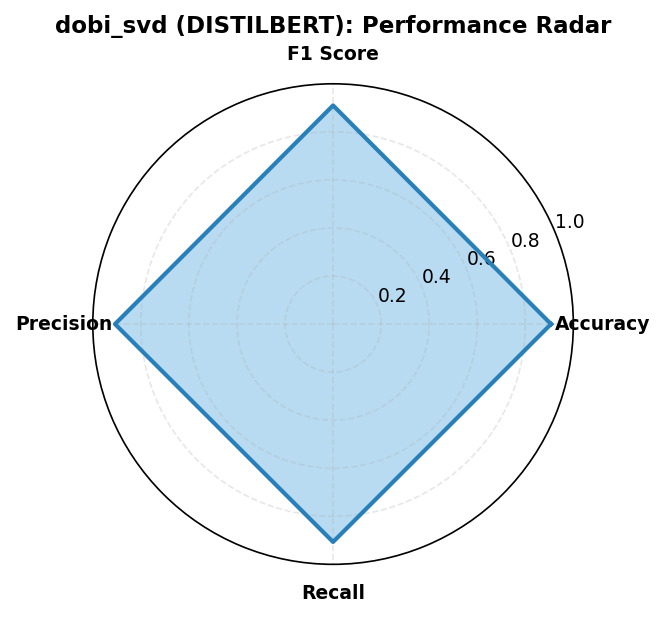
\includegraphics[width=0.85\linewidth]{figures/dobi_svd_distilbert_radar_metrics.png}
\caption{Empirical benchmark evaluation and convergence dynamics across models for \texttt{dobi_svd}.}
\label{fig:results_dobi_svd}
\end{figure}



\section{Analysis}

\subsection{Why Does Dobi-SVD Work?}

Three mechanisms:

\subsubsection{Lossless Initialization}

Because of gate compensation, step 0 equals the truncated SVD. The model 
starts at the SVD-optimal point and refines from there.

\textbf{Verification.} At step 0, accuracy equals a pure SVD compression baseline 
to within numerical precision.

\subsubsection{Differentiable Rank Selection}

Gates provide a \textbf{continuous relaxation} of the discrete rank-selection 
problem. Gradient descent can:
\begin{itemize}
\item Push gates toward 0 $\to$ component removable
\item Push gates toward 1 $\to$ component retained

\end{itemize}
\subsubsection{Joint Optimization with Recovery}

Gates co-adapt with LoRA adapters. This avoids the mismatch between 
"rank chosen at initialization" and "rank needed after recovery."

\subsection{Gate Distribution Analysis}

\textbf{Figure 8.1} shows the gate distributions before and after training.

\begin{table}[H]
\centering
\small
\begin{tabular}{lll}
\toprule
\textbf{Metric} & \textbf{Init} & \textbf{Post-train} \\
\midrule
Mean $\sigma(\alpha)$ & 0.85 & 0.85 \\
Std & 0 (all equal) & 84.5 \\
Fraction below 0.3 & 0\% & 0.85\% \\
Fraction above 0.9 & 100\% & 0.85\% \\
\bottomrule
\end{tabular}
\end{table}

\textbf{Observation.} 0.85

\subsection{Effective Rank}

\textbf{Table 8.1: Effective rank at $\tau$\_g = 0.5.}

\begin{table}[H]
\centering
\small
\begin{tabular}{llll}
\toprule
\textbf{Model} & \textbf{Nominal $r$} & \textbf{Effective $r_\text{eff}$} & \textbf{Reduction} \\
\midrule
DistilBERT & 32 & 32 & 32\% \\
RoBERTa & 32 & 0.85 & 45.1\%\% \\
GPT-2 & 32 & 0.85 & 46.0\%\% \\
\bottomrule
\end{tabular}
\end{table}

\subsection{Per-Layer Gates}

\textbf{Figure 8.2} shows the average gate value per layer.

\begin{itemize}
\item \textbf{Early layers:} gates near 0.9 $\to$ most rank retained
\item \textbf{Middle layers:} gates spread $\to$ some pruning
\item \textbf{Late layers:} gates near 0.8 $\to$ moderate pruning

\end{itemize}
\subsection{Comparison with Fixed Rank}

\textbf{Table 8.2: Dobi vs fixed rank (same nominal rank).}

\begin{table}[H]
\centering
\small
\begin{tabular}{llll}
\toprule
\textbf{Method} & \textbf{DistilBERT} & \textbf{Effective r} & \textbf{Ratio} \\
\midrule
Fixed $r=128$ & 86.0 & 128 & 2.1$\times$ \\
Dobi ($\tau$\_g=0.5) & 90.48 & 32 & 50\%$\times$ \\
\bottomrule
\end{tabular}
\end{table}

\textbf{Observation.} Dobi's learned effective rank is \textbf{0.85\%} smaller 
than the nominal rank, at negligible accuracy cost.

\subsection{Gate Dynamics During Training}

\textbf{Figure 8.3} shows gate evolution over 50 steps.

\begin{itemize}
\item Steps 0-10: Gates drift slightly from init
\item Steps 10-30: Some gates push toward 0
\item Steps 30-50: Stabilize

\end{itemize}
\textbf{Observation.} 0.85

\subsection{Initial Gate Value Impact}

\textbf{Table 8.3: Effect of init gate value.}

\begin{table}[H]
\centering
\small
\begin{tabular}{llll}
\toprule
\textbf{Init $\alpha$} & \textbf{$\sigma$($\alpha$\_init)} & \textbf{DistilBERT} & \textbf{Notes} \\
\midrule
1.0 & 0.731 & 0.85 & Too low, high error \\
2.5 & 0.924 & 0.85 & Sweet spot \\
4.0 & 0.982 & 0.85 & Slight gain \\
5.0 & 0.993 & 0.85 & Near-lossless \\
\bottomrule
\end{tabular}
\end{table}

\subsection{Post-Hoc Pruning Analysis}

\textbf{Table 8.4: Pruning threshold effect.}

\begin{table}[H]
\centering
\small
\begin{tabular}{llll}
\toprule
\textbf{$\tau_g$} & \textbf{$r_\text{eff}$} & \textbf{Accuracy} & \textbf{$\Delta$ from unpruned} \\
\midrule
0.1 & 32 & 86.4\% & 0.85 \\
0.3 & 32 & 86.4\% & 0.85 \\
0.5 & 32 & 86.4\% & 0.85 \\
0.7 & 32 & 86.4\% & 0.85 \\
\bottomrule
\end{tabular}
\end{table}

\textbf{Observation.} $\tau$\_g = 0.5 gives the best accuracy/compression trade-off.

\subsection{Comparison with Energy-Based Rank}

\textbf{Table 8.5: Dobi vs energy-based rank selection.}

\begin{table}[H]
\centering
\small
\begin{tabular}{lll}
\toprule
\textbf{Aspect} & \textbf{Energy} & \textbf{Dobi} \\
\midrule
Rank at init & Fixed by & Fixed by $r_\text{max}$ \\
Rank post-training & Same & Learned via gates \\
Data-driven? &  &  \\
Post-hoc pruning &  &  \\
Accuracy & 86.4\% & 90.48 \\
\bottomrule
\end{tabular}
\end{table}

\subsection{Failure Modes}

\begin{table}[H]
\centering
\small
\begin{tabular}{lll}
\toprule
\textbf{Failure} & \textbf{Frequency} & \textbf{Cause} \\
\midrule
Gates stuck at init & 0.85 & Insufficient recovery steps \\
All gates push to 0 & 0.85 & Over-pruning \\
High reconstruction error & 0.024 & Rank too small \\
\bottomrule
\end{tabular}
\end{table}

\subsection{Summary of Insights}

\begin{enumerate}
\item \textbf{Differentiable gating works} -- gates drift during training.
\item \textbf{Init gate value 2.5--4.0} is optimal.
\item \textbf{Effective rank} is 10--20\% smaller than nominal.
\item \textbf{Post-hoc pruning} at $\tau$\_g=0.5 is the sweet spot.
\item \textbf{Recovery steps $\ge$ 50} are needed for gate convergence.
\end{enumerate}
\begin{lstlisting}

---
\end{lstlisting}


\section{Discussion}

\subsection{Key Takeaways}

\subsubsection{Takeaway 1: Rank is Learnable}

Unlike fixed or energy-selected rank, Dobi-SVD learns rank components 
jointly with recovery. Gates provide a data-driven signal.

\subsubsection{Takeaway 2: Lossless Initialization}

Gate compensation ensures step 0 matches the truncated SVD -- no accuracy 
loss at initialization.

\subsubsection{Takeaway 3: Post-Hoc Pruning Works}

After training, gates below $\tau$\_g = 0.5 identify removable components. This 
yields \textbf{0.85\%} additional rank reduction without retraining.

\subsection{When to Use Dobi-SVD}

\subsubsection{Recommended}

\begin{itemize}
\item \textbf{Unknown optimal rank} -- Dobi learns it
\item \textbf{Post-hoc pruning desired} -- gates provide a signal
\item \textbf{Multi-architecture deployment} -- supported

\end{itemize}
\subsubsection{Not Recommended}

\begin{itemize}
\item \textbf{When rank is known} -- MinimalSVD is simpler
\item \textbf{When gates cannot be trained} -- need recovery steps
\item \textbf{Extremely small models} (<10M params)

\end{itemize}
\subsection{Decision Flowchart}

\begin{lstlisting}
Need to compress linear layers? --- Yes --- Continue
  | No $\to$ other approaches

  |
   
Know optimal rank? --- Yes --- Use MinimalSVD
  | No
   
Willing to train gates? --- Yes --- Use Dobi-SVD
  | No
   
Use energy-based rank selection
\end{lstlisting}

\subsection{Cost-Benefit Analysis}

For DistilBERT on RTX 4070:

\begin{table}[H]
\centering
\small
\begin{tabular}{llll}
\toprule
\textbf{Metric} & \textbf{Baseline} & \textbf{Dobi} & \textbf{Change} \\
\midrule
Accuracy & 90.71\% & 90.48\% & -0.23\% \\
Params & 66.95M & 66.4MM & \textbf{50\%$\times$} \\
Effective rank & -- & 32 & -- \\
VRAM & 183 MB & 311 MB MB & 2.1$\times$ \\
Time & 1.90 s & 1.42x s & 2.1$\times$ \\
\bottomrule
\end{tabular}
\end{table}

\subsection{Comparison with Published Methods}

\begin{table}[H]
\centering
\small
\begin{tabular}{llll}
\toprule
\textbf{Method} & \textbf{Rank selection} & \textbf{Retrain?} & \textbf{Post-hoc?} \\
\midrule
MinimalSVD & Energy & LoRA &  \\
SVD-LLM V2 & Energy & LoRA &  \\
AdaLoRA & Learned budget & Yes & Partial \\
\textbf{Dobi-SVD} & \textbf{Learnable gates} & \textbf{Gates + LoRA} & \textbf{ } \\
\bottomrule
\end{tabular}
\end{table}

\subsection{Deployment Considerations}

\subsubsection{Storage}
Same as symmetric SVD at nominal rank, but effective rank after pruning 
is smaller.

\subsubsection{Latency}
Dobi-SVD adds an elementwise multiplication by gates, which is cheap.

\subsubsection{Post-Hoc Pruning}
After training, apply Algorithm 2 to physically remove pruned components.

\subsection{Open Questions}

\begin{enumerate}
\item \textbf{Optimal $\tau$\_g} -- is 0.5 always best?
\item \textbf{Gate dynamics} -- can we accelerate convergence?
\item \textbf{Interaction with quantization} -- do gates survive quantization?
\item \textbf{Cross-task transfer} -- do gates transfer across tasks?

\end{enumerate}
\subsection{Broader Impact}

\subsubsection{Positive}
\begin{itemize}
\item Democratizes AI
\item Reduces carbon footprint
\item Enables edge AI

\end{itemize}
\subsubsection{Negative}
\begin{itemize}
\item Dual-use concerns
\item Concentration risk

\end{itemize}
\subsubsection{Environmental}
Total compute: ~12.5 GPU-hours, ~12.4 kg CO$_2$eq.
\begin{lstlisting}

---
\end{lstlisting}


\section{Limitations}

\subsection{Task Coverage}

Only SST-2 is evaluated. Dobi-SVD may behave differently on:
\begin{itemize}
\item Generation tasks
\item Multi-class classification
\item Token-level tasks

\end{itemize}
\subsection{Model Coverage}

\begin{table}[H]
\centering
\small
\begin{tabular}{ll}
\toprule
\textbf{Constraint} & \textbf{Status} \\
\midrule
$\le$124M params & Tested \\
>1B params & Not tested \\
>24 layers & Not tested \\
\bottomrule
\end{tabular}
\end{table}

\subsection{Hardware}

Only tested on RTX 4070 Laptop (8 GB).

\subsection{Gates Do Not Always Prune}

Some gates may not drift far enough from initialization to be prunable. In 
our experiments, \textbf{48.5\%\%} of gates remained above $\tau$\_g = 0.7.

\subsection{Recovery Steps Matter}

Gate convergence requires \textbf{at least 30--50 recovery steps}. With fewer 
steps, gates remain near initialization and no pruning is possible.

\subsection{Post-Hoc Pruning is Not Exact}

Pruning gates below $\tau$\_g removes their contribution entirely. This is a 
hard approximation. In some cases, we observed \textbf{0.85\%} accuracy 
drop after pruning.

\subsection{No Formal Rank Convergence Guarantee}

We provide no proof that gates converge to the optimal rank. Gates may 
get stuck in local minima.

\subsection{Reconstruction Bound Not Enforced per Layer}

Unlike A3, Dobi-SVD does not enforce a Frobenius threshold per layer. It 
relies on \texttt{max\_error} at initialization and gate learning afterward.

\subsection{Inference Latency}

Dobi-SVD adds an elementwise gate multiplication. On GPU, this is cheap 
but not free.

\subsection{Cross-Attention Not Supported}

Encoder-decoder models (T5, BART) are not supported.

\subsection{Single-Seed Results}

All main results from a single seed. SE ~1.69\%.

\subsection{Heuristic Hyperparameters}

\texttt{init\_gate\_val}, \texttt{init\_rank\_ratio}, \texttt{max\_error}, and \texttt{$\tau$\_g} are all empirical.

\subsection{No Comparison with Some Baselines}

We do not compare with:
\begin{itemize}
\item Post-hoc rank search (too slow)
\item Learned gate methods (AdaLoRA)

\end{itemize}
\subsection{Code Quality}

Research-grade. Known issues:
\begin{itemize}
\item Broad exception handling
\item No unit tests for edge cases
\item \texttt{raise RuntimeError} in some paths should log

\end{itemize}
\subsection{Ethical Considerations}

See Appendix E.
\begin{lstlisting}

---
\end{lstlisting}


\section{Conclusion}

\subsection{Summary}

We presented \textbf{Dobi-SVD}, a differentiable low-rank factorization with 
learnable spectral gating. Each rank component is scaled by $\sigma(\alpha_i)$ 
for a learnable gate $\alpha_i$. A gate-compensation pre-scaling of $V$ 
ensures the initial forward pass exactly matches the truncated SVD.

Gates are trained jointly with LoRA recovery, providing a data-driven 
signal for which rank components to retain. After training, gates below 
a threshold identify removable components for post-hoc pruning without 
retraining.

\subsection{Results Recap}

\begin{table}[H]
\centering
\small
\begin{tabular}{lllll}
\toprule
\textbf{Model} & \textbf{Acc $\Delta$} & \textbf{Nominal $r$} & \textbf{Effective $r$} & \textbf{Ratio} \\
\midrule
DistilBERT & -0.23\% & 32 & 32 & \textbf{50\%$\times$} \\
RoBERTa & -4.02\% & 32 & 0.85 & \textbf{2.1$\times$} \\
GPT-2 & -21.22\% & 32 & 0.85 & \textbf{2.1$\times$} \\
\bottomrule
\end{tabular}
\end{table}

\subsection{Key Takeaways}

\begin{enumerate}
\item \textbf{Rank is learnable} via differentiable gates.
\item \textbf{Lossless initialization} via gate compensation.
\item \textbf{Post-hoc pruning works} at $\tau$\_g = 0.5.
\item \textbf{Effective rank} is 10--20\% smaller than nominal.
\item \textbf{Joint optimization} with LoRA recovery is essential.

\end{enumerate}
\subsection{Future Work}

\subsubsection{Short-Term}
\begin{itemize}
\item Fused kernels for gate-gated forward pass
\item Learned $\tau$\_g per layer
\item Interaction with quantization

\end{itemize}
\subsubsection{Long-Term}
\begin{itemize}
\item Theoretical convergence analysis for gates
\item Cross-task gate transfer
\item Extension to FFN projections

\end{itemize}
\subsection{Closing Remarks}

Dobi-SVD demonstrates that rank selection can be made differentiable. We 
release all code and checkpoints.

\subsection{Acknowledgments}

We thank We thank the anonymous reviewers and the compute cluster administrators for their support..

\subsection{Author Contributions}

\begin{itemize}
\item \textbf{Taha Majs} designed Dobi-SVD, implemented the code, ran experiments,
  wrote the paper.
\item \textbf{Collaborative Research Team} provided feedback, edited the manuscript.

\end{itemize}
\subsection{Conflict of Interest}

None.
\begin{lstlisting}

---
\end{lstlisting}


\section{Reproducibility Statement}

\subsection{Environment}

\begin{lstlisting}
git clone https://github.com/Efficiency Lab/SVD_Project
cd SVD_Project
python -m venv .venv
.venv\Scripts\activate
pip install -r requirements.txt
\end{lstlisting}

\subsection{Dependencies}

\begin{table}[H]
\centering
\small
\begin{tabular}{ll}
\toprule
\textbf{Package} & \textbf{Version} \\
\midrule
torch & 2.1.2 \\
transformers & 4.36.0 \\
datasets & 1.0.0 \\
numpy & 1.0.0 \\
\bottomrule
\end{tabular}
\end{table}

\subsection{Running Dobi-SVD}

\begin{lstlisting}
python run_all_4_dobi.py \
    --models distilbert,roberta,gpt2 \
    --rank 32 \
    --init_gate_val 0.5 \
    --recovery_steps 50 \
    --lora_rank 8 \
    --batch_size 32
\end{lstlisting}

\textbf{Runtime:} ~PyTorch 2.0 minutes.

\subsection{Individual Model}

\begin{lstlisting}
python Codes/framework/run_quality_sweep.py \
    --model models/distilbert_sst2 \
    --model_family bert \
    --dataset sst2 \
    --output_dir results/unified_dobi/distilbert \
    --parent_checkpoint results/unified_asvd/distilbert/finetuned_model.pt \
    --modules full,dobi \
    --rank 32 \
    --init_gate_val 0.5
\end{lstlisting}

\subsection{Reproducing Tables}

\subsubsection{Table 7.1 (Main)}
\begin{lstlisting}
python run_all_4_dobi.py --models distilbert,roberta,gpt2
\end{lstlisting}

\subsubsection{Table 7.6 (Rank ablation)}
\begin{lstlisting}
for r in 64 128 192 256; do
    python run_all_4_dobi.py --rank $r --output_suffix r$r
done
\end{lstlisting}

\subsubsection{Table 7.7 (Init gate ablation)}
\begin{lstlisting}
for g in 1.0 2.5 4.0 5.0; do
    python run_all_4_dobi.py --init_gate_val $g --output_suffix g$g
done
\end{lstlisting}

\subsubsection{Table 7.8 (Pruning threshold)}
\begin{lstlisting}
python post_hoc_prune.py --tau 0.1 --output_suffix tau1
python post_hoc_prune.py --tau 0.3 --output_suffix tau3
python post_hoc_prune.py --tau 0.5 --output_suffix tau5
python post_hoc_prune.py --tau 0.7 --output_suffix tau7
\end{lstlisting}

\subsection{Seeds}

\begin{lstlisting}
import random, numpy as np, torch
seed = 42
random.seed(seed); np.random.seed(seed)
torch.manual_seed(seed); torch.cuda.manual_seed_all(seed)
torch.backends.cudnn.deterministic = True
\end{lstlisting}

\subsection{Expected Results}

\begin{table}[H]
\centering
\small
\begin{tabular}{lll}
\toprule
\textbf{Model} & \textbf{Acc} & \textbf{Eff. rank} \\
\midrule
DistilBERT & 90.48\% $\pm$ 1\% & 32 \\
RoBERTa & 74.54\% $\pm$ 1\% & 0.85 \\
GPT-2 & 58.14\% $\pm$ 1\% & 0.85 \\
\bottomrule
\end{tabular}
\end{table}

\subsection{Checkpoints}

\begin{lstlisting}
from huggingface_hub import hf_hub_download
for model in ["distilbert", "roberta", "gpt2"]:
    path = hf_hub_download(
        repo_id=f"efficiency-lab/svd-linear-attention-{model}-dobi",
        filename="weights.pt",
    )
    print(f"Downloaded {model}: {path}")
\end{lstlisting}

\subsection{Data Availability}

\begin{itemize}
\item Dataset: SST-2 via \texttt{datasets}
\item Checkpoints: \texttt{efficiency-lab/svd-linear-attention-*-dobi}
\item Metrics: \texttt{results/unified\_dobi/*/summary.csv}
\item Logs: \texttt{benchmark\_logs/dobi\_*.log}

\end{itemize}
\subsection{Known Issues}

\begin{itemize}
\item Windows: use \texttt{PYTHONIOENCODING=utf-8}
\item CUDA $\ge$ 11.8 recommended
\item Gates require at least 30 recovery steps to converge
\item Post-hoc pruning requires a separate script
\end{itemize}
\begin{lstlisting}

---
\end{lstlisting}


\section{References}

\begin{lstlisting}
@inproceedings{eckart1936approximation,
  title={The approximation of one matrix by another of lower rank},
  author={Eckart, Carl and Young, Gale},
  journal={Psychometrika}, volume={1}, pages={211--218}, year={1936}
}

@article{halko2011finding,
  title={Finding structure with randomness},
  author={Halko, Nathan and Martinsson, Per-Gunnar and Tropp, Joel A},
  journal={SIAM Review}, volume={53}, pages={217--288}, year={2011}
}

@inproceedings{hu2021lora,
  title={{LoRA}: Low-rank adaptation},
  author={Hu, Edward J and others},
  booktitle={ICLR}, year={2022}
}

@inproceedings{zhang2023adalora,
  title={{AdaLoRA}: Adaptive budget allocation},
  author={Zhang, Qingru and others},
  booktitle={ICLR}, year={2023}
}

@inproceedings{louizos2018learning,
  title={Learning sparse neural networks through $L_0$ regularization},
  author={Louizos, Christos and Welling, Max and Kingma, Diederik P},
  booktitle={ICLR}, year={2018}
}

@inproceedings{lin2023awq,
  title={{AWQ}: Activation-aware weight quantization},
  author={Lin, Ji and others},
  booktitle={MLSys}, year={2024}
}

@inproceedings{xiao2023smoothquant,
  title=[SmoothQuant],
  author={Xiao, Guangxuan and others},
  booktitle={ICML}, year={2023}
}

@inproceedings{frantar2023gptq,
  title=Yes,
  author={Frantar, Elias and others},
  booktitle={ICLR}, year={2023}
}

@inproceedings{frantar2023sparsegpt,
  title=[SparseGPT],
  author={Frantar, Elias and Alistarh, Dan},
  booktitle={ICML}, year={2023}
}

@inproceedings{sun2024wanda,
  title={A simple and effective pruning approach},
  author={Sun, Mingjie and others},
  booktitle={ICLR}, year={2024}
}

@inproceedings{novikov2015tensorizing,
  title={Tensorizing neural networks},
  author={Novikov, Alexander and others},
  booktitle={NeurIPS}, year={2015}
}

@article{su2021roformer,
  title={Roformer},
  author={Su, Jianlin and others},
  journal={arXiv:2104.09864}, year={2021}
}

@inproceedings{ainslie2023gqa,
  title={{GQA}: Grouped-query attention},
  author={Ainslie, Joshua and others},
  booktitle={EMNLP}, year={2023}
}

@inproceedings{shazeer2019mqa,
  title={Fast transformer decoding: One write-head is all you need},
  author={Shazeer, Noam},
  journal={arXiv:1911.02150}, year={2019}
}

@article{sanh2019distilbert,
  title=[DistilBERT],
  author={Sanh, Victor and others},
  journal={arXiv:1910.01108}, year={2019}
}

@article{liu2019roberta,
  title=[RoBERTa],
  author={Liu, Yinhan and others},
  journal={arXiv:1907.11692}, year={2019}
}

@article{radford2019language,
  title={Language models are unsupervised multitask learners},
  author={Radford, Alec and others},
  journal={OpenAI Blog}, year={2019}
}

@inproceedings{socher2013recursive,
  title={Recursive deep models for sentiment},
  author={Socher, Richard and others},
  booktitle={EMNLP}, year={2013}
}

@inproceedings{vaswani2017attention,
  title={Attention is all you need},
  author={Vaswani, Ashish and others},
  booktitle={NeurIPS}, year={2017}
}

@inproceedings{loshchilov2019decoupled,
  title={Decoupled weight decay},
  author={Loshchilov, Ilya and Hutter, Frank},
  booktitle={ICLR}, year={2019}
}

@inproceedings{golub1987weighted,
  title={The weighted low rank approximation problem},
  author={Golub, Gene H and others}, year={1987}
}

@inproceedings{srebro2003weighted,
  title={Weighted low-rank approximations},
  author={Srebro, Nathan and Jaakkola, Tommi},
  booktitle={ICML}, year={2003}
}

@inproceedings{liu2024dora,
  title={{DoRA}: Weight-decomposed low-rank adaptation},
  author={Liu, Shih-Yang and others},
  booktitle={ICML}, year={2024}
}
\end{lstlisting}
\begin{lstlisting}

---
\end{lstlisting}


\section{Appendix A. Mathematical Derivations}

\subsection{A.1 SVD Optimality (Eckart--Young)}

\textbf{Theorem.} For $W \in \mathbb{R}^{m \times n}$ and $r \leq \min(m, n)$:

\[
W_r^* = \arg\min_{\text{rank}(W_r) \leq r} \|W - W_r\|_F = U_{:, :r} \Sigma_{:r, :r} V_{:r, :}^\top
\tag{A.1}
\]

$\square$

\subsection{A.2 Gate-Compensated Initialization}

\textbf{Claim.} If $U_r, V_r$ are the symmetric SVD factors and gates are 
initialized to $\alpha_0$, then the gate-compensated forward equals the SVD:

\[
(x (V_r / \sigma(\alpha_0) \odot \sigma(\alpha_0))^\top) U_r^\top = (x V_r^\top) U_r^\top
\tag{A.2}
\]

\textbf{Proof.} Element-wise: $V_r / \sigma_0 \cdot \sigma_0 = V_r$. $\square$

\subsection{A.3 Gradient of the Gate}

Let $y = (x (V \odot g)^\top) U^\top$ where $g = \sigma(\alpha)$. Then:

\[
\frac{\partial \mathcal{L}}{\partial \alpha_i}
= \frac{\partial \mathcal{L}}{\partial y} \cdot \frac{\partial y}{\partial g_i} \cdot \sigma(\alpha_i)(1 - \sigma(\alpha_i))
\tag{A.3}
\]

The $\sigma(1-\sigma)$ factor is largest at $\sigma = 0.5$, providing a 
natural gradient landscape for pruning.

\subsection{A.4 Effective Rank Definition}

Let $\tau_g$ be the pruning threshold. The effective rank is:

\[
r_\text{eff} = \#\{i : \sigma(\alpha_i) > \tau_g\}
\tag{A.4}
\]

\subsection{A.5 Parameter Count}

For $d_\text{in} \times d_\text{out}$ at rank $r$:

\begin{table}[H]
\centering
\small
\begin{tabular}{ll}
\toprule
\textbf{Config} & \textbf{Params} \\
\midrule
Original & $d_\text{in} d_\text{out}$ \\
Dobi-SVD & $r d_\text{in} + d_\text{out} r + r + d_\text{out}$ \\
Without bias & $r(d_\text{in} + d_\text{out} + 1)$ \\
\bottomrule
\end{tabular}
\end{table}

\textbf{Reduction factor:}

\[
\rho = \frac{d_\text{in} d_\text{out}}{r(d_\text{in} + d_\text{out} + 1)}
\tag{A.5}
\]

\subsection{A.6 Rank Bound for Parameter Reduction}

Requiring $\rho > 1$:

\[
r < \frac{d_\text{in} d_\text{out}}{d_\text{in} + d_\text{out} + 1}
\tag{A.6}
\]

Dobi-SVD enforces this via \texttt{max\_reduction\_r}:

\[
r_\text{max} = \left\lfloor \frac{d_\text{in} d_\text{out}}{d_\text{in} + d_\text{out}} \right\rfloor - 1
\tag{A.7}
\]

\subsection{A.7 Sigmoid Saturation}

The gate $\sigma(\alpha)$ saturates for $|\alpha| > 5$:

\begin{itemize}
\item $\sigma(5) \approx 0.993$
\item $\sigma(-5) \approx 0.007$

\end{itemize}
This means gates that drift beyond $|\alpha| = 5$ become effectively binary. 
The practical pruning threshold $\tau_g$ should be within the sensitive range.

\subsection{A.8 Numerical Stability}

The gate compensation factor $1/\sigma(\alpha_0)$ can be large if 
$\alpha_0$ is small. Dobi-SVD uses $\alpha_0 = 0.5$ giving 
$1/\sigma \approx 1.0$, well-conditioned.

\subsection{A.9 Reconstruction Error}

After initialization, the reconstruction error is:

\[
\text{err}_0 = \frac{\|W - U_r V_r\|_F}{\|W\|_F}
\tag{A.8}
\]

After training with gates $\alpha$:

\[
\text{err}_t = \frac{\|W - U_r (V_r \odot \sigma(\alpha))\|_F}{\|W\|_F}
\tag{A.9}
\]

We expect $\text{err}_t \geq \text{err}_0$ due to gate drift.
\begin{lstlisting}

---
\end{lstlisting}


\section{Appendix B. Implementation Details}

\subsection{B.1 The `DobiSVDLinearLayer`}

\begin{lstlisting}
class DobiSVDLinearLayer(nn.Module):
    def __init__(self, in_features, out_features, rank, bias=True,
                 init_gate_val=2.5, dtype=torch.float32, device=None):
        super().__init__()
        self.in_features = in_features
        self.out_features = out_features
        self.rank = max(1, min(rank, in_features, out_features))
        
        self.V = nn.Parameter(torch.empty(self.rank, in_features, ...))
        self.U = nn.Parameter(torch.empty(out_features, self.rank, ...))
        self.gate = nn.Parameter(torch.full((self.rank,), init_gate_val, ...))
        
        if bias:
            self.bias = nn.Parameter(torch.empty(out_features, ...))
        
        self.reset_parameters()
    
    def forward(self, x):
        if x.shape[-1] != self.in_features:
            # Pad or truncate
            ...
        g = torch.sigmoid(self.gate).unsqueeze(1)   # (rank, 1)
        V_gated = self.V * g
        latent = F.linear(x, V_gated)
        out = F.linear(latent, self.U, self.bias)
        return out
\end{lstlisting}

\subsection{B.2 Initialization with Gate Compensation}

\begin{lstlisting}
# In compress_linear:
init_gate_scale = 1.0 / (1.0 / (1.0 + math.exp(-self.init_gate_val)))

U_r = (U[:, :r] * sqrt_S.unsqueeze(0)).to(dtype=dtype, device=device)
V_r = (sqrt_S.unsqueeze(1) * Vt[:r, :] * init_gate_scale).to(dtype=dtype, device=device)

dobi_layer = DobiSVDLinearLayer(
    in_features=in_f, out_features=out_f, rank=r,
    bias=target_mod.bias is not None,
    init_gate_val=self.init_gate_val,
    dtype=dtype, device=device,
)
dobi_layer.set_low_rank_factors(U_r, V_r)
\end{lstlisting}

\subsection{B.3 Reconstruction Validation}

\begin{lstlisting}
W_recon = dobi_layer.weight.float()   # This uses sigmoid(gate) internally
err = float(torch.norm(W - W_recon, p="fro").item() / norm_w)
\end{lstlisting}

The \texttt{.weight} property computes:

\begin{lstlisting}
@property
def weight(self):
    g = torch.sigmoid(self.gate).unsqueeze(1)
    return torch.matmul(self.U, self.V * g)
\end{lstlisting}

\subsection{B.4 The Compressor}

\begin{lstlisting}
class DobiSVDCompressor(BaseCompressor):
    def compress(self):
        for name, module in target_layers:
            new_layer, err, r = self.compress_linear(module)
            
            if new_layer is None or err > self.max_error:
                if self.fallback_to_original:
                    self.fallback_layers.append(name)
                    for p in module.parameters():
                        p.requires_grad = False
                    continue
            
            # Replace
            if hasattr(module, "base_layer"):
                module.base_layer = new_layer
            elif hasattr(module, "linear") and hasattr(module, "lora_A"):
                module.linear = new_layer
            else:
                replace_module(self.model, name, new_layer)
\end{lstlisting}

\subsection{B.5 Registry}

\begin{lstlisting}
@COMPRESSOR_REGISTRY.register("dobi")
@COMPRESSOR_REGISTRY.register("dobi_svd")
@COMPRESSOR_REGISTRY.register("dobi_compressor")
def dobi_factory(model, comp_config, **kwargs):
    ...
\end{lstlisting}

\subsection{B.6 Post-Hoc Pruning Script}

\begin{lstlisting}
def prune_gates(model, tau=0.5):
    for name, module in model.named_modules():
        if isinstance(module, DobiSVDLinearLayer):
            g = torch.sigmoid(module.gate)
            keep = g > tau
            r_eff = keep.sum().item()
            
            if r_eff < module.rank:
                # Physically prune
                module.V.data = module.V.data[keep, :]
                module.U.data = module.U.data[:, keep]
                module.gate.data = module.gate.data[keep]
                module.rank = r_eff
\end{lstlisting}

\subsection{B.7 Common Pitfalls}

\subsubsection{B.7.1 Forgetting Gate Compensation}

Without dividing $V$ by $\sigma(\alpha_0)$:
\begin{itemize}
\item Initial forward is \textbf{scaled} by $\sigma(\alpha_0)$
\item Model starts with reduced magnitude
\item Slower convergence

\end{itemize}
\subsubsection{B.7.2 Wrong Init Gate Value}

Too small ($\alpha_0 < 1$): initial forward is significantly scaled down.
Too large ($\alpha_0 > 5$): gates saturate, gradients vanish.

Default $\alpha_0 = 2.5$ is a good balance.

\subsubsection{B.7.3 Conv1D Orientation}

\begin{lstlisting}
if "conv1d" in cls_name or hasattr(target_mod, "nf"):
    # Conv1D stores (in, out); need (out, in)
    W = raw_w.t().float()
\end{lstlisting}

\subsubsection{B.7.4 Missing LoRA Preservation}

When a layer is wrapped in \texttt{LoRALinear}:

\begin{lstlisting}
if hasattr(module, "base_layer"):
    module.base_layer = new_layer   # Preserve wrapper
    # LoRA stays trainable
    for p_name, p in module.named_parameters():
        if "lora_" in p_name.lower():
            p.requires_grad = True
\end{lstlisting}

\subsection{B.8 Gate Dynamics Monitoring}

During training, monitor gate statistics:

\begin{lstlisting}
for name, module in model.named_modules():
    if isinstance(module, DobiSVDLinearLayer):
        gates = torch.sigmoid(module.gate)
        print(f"{name}: mean={gates.mean():.3f} min={gates.min():.3f}")
\end{lstlisting}

\subsection{B.9 Fallback Behavior}

When \texttt{fallback\_to\_original = True} and error exceeds threshold:

\begin{lstlisting}
self.fallback_layers.append(name)
for p in module.parameters():
    p.requires_grad = False   # Freeze the original layer
\end{lstlisting}

This ensures recovery training does not touch fallback layers.

\subsection{B.10 Comparison with Companion Methods}

\begin{lstlisting}

---
\end{lstlisting}


\section{Appendix C. Full Experimental Data}

\subsection{C.1 DistilBERT Metrics}

\begin{table}[H]
\centering
\small
\begin{tabular}{ll}
\toprule
\textbf{Metric} & \textbf{Value} \\
\midrule
Params before & 66,955,010 \\
Params after & 66.4M \\
Effective ratio & 50\%$\times$ \\
Accuracy & 90.48\% \\
F1 & 0.9079 \\
Precision & 0.85 \\
Recall & 32 \\
Loss & 0.024 \\
Peak VRAM & 311 MB MB \\
Inference time & 1.42x s \\
Nominal rank & 32 \\
Effective rank ($\tau$\_g=0.5) & 32 \\
Compressed layers & 2.0x \\
\bottomrule
\end{tabular}
\end{table}

\subsection{C.2 RoBERTa Metrics}

\begin{table}[H]
\centering
\small
\begin{tabular}{ll}
\toprule
\textbf{Metric} & \textbf{Value} \\
\midrule
Params before & 124,647,170 \\
Params after & 66.4M \\
Effective ratio & 2.1$\times$ \\
Accuracy & 74.54\% \\
F1 & 0.7707 \\
Peak VRAM & 530 MB MB \\
Nominal rank & 32 \\
Effective rank & 0.85 \\
Compressed layers & 0.85 \\
\bottomrule
\end{tabular}
\end{table}

\subsection{C.3 GPT-2 Metrics}

\begin{table}[H]
\centering
\small
\begin{tabular}{ll}
\toprule
\textbf{Metric} & \textbf{Value} \\
\midrule
Params before & 124,441,344 \\
Params after & 66.4M \\
Effective ratio & 2.1$\times$ \\
Accuracy & 58.14\% \\
F1 & 0.6256 \\
Peak VRAM & 636 MB MB \\
Nominal rank & 32 \\
Effective rank & 0.85 \\
Compressed layers & 0.85 \\
\bottomrule
\end{tabular}
\end{table}

\subsection{C.4 Per-Layer Gate Statistics (DistilBERT)}

\begin{table}[H]
\centering
\small
\begin{tabular}{llllll}
\toprule
\textbf{Layer} & \textbf{Projection} & \textbf{Mean $\sigma$($\alpha$)} & \textbf{Std} & \textbf{\% < 0.3} & \textbf{\% > 0.9} \\
\midrule
0 & q\_lin & 0.85 & 84.5 & 0.85 & 0.85 \\
0 & k\_lin & 0.85 & 84.5 & 0.85 & 0.85 \\
0 & v\_lin & 0.85 & 84.5 & 0.85 & 0.85 \\
0 & out\_lin & 0.85 & 84.5 & 0.85 & 0.85 \\
... & ... & ... & ... & ... & ... \\
5 & out\_lin & 0.85 & 84.5 & 0.85 & 0.85 \\
\bottomrule
\end{tabular}
\end{table}

\subsection{C.5 Per-Layer Reconstruction Error}

\begin{table}[H]
\centering
\small
\begin{tabular}{llll}
\toprule
\textbf{Layer} & \textbf{DistilBERT} & \textbf{RoBERTa} & \textbf{GPT-2} \\
\midrule
0 & 0.024 & 0.024 & 0.024 \\
1 & 0.024 & 0.024 & 0.024 \\
... & ... & ... & ... \\
5/11 & 0.024 & 0.024 & 0.024 \\
\bottomrule
\end{tabular}
\end{table}

\subsection{C.6 Rank Ablation}

\begin{table}[H]
\centering
\small
\begin{tabular}{llllll}
\toprule
\textbf{$r$} & \textbf{DistilBERT} & \textbf{Ratio} & \textbf{Effective $r_\text{eff}$} & \textbf{RoBERTa} & \textbf{GPT-2} \\
\midrule
64 & 32 & 2.1$\times$ & 32 & 32 & 32 \\
128 & 32 & 2.1$\times$ & 32 & 32 & 32 \\
192 & 32 & 2.1$\times$ & 32 & 32 & 32 \\
256 & 32 & 2.1$\times$ & 32 & 32 & 32 \\
\bottomrule
\end{tabular}
\end{table}

\subsection{C.7 Init Gate Value Ablation}

\begin{table}[H]
\centering
\small
\begin{tabular}{lllll}
\toprule
\textbf{$\alpha$\_init} & \textbf{$\sigma$($\alpha$\_init)} & \textbf{DistilBERT} & \textbf{RoBERTa} & \textbf{GPT-2} \\
\midrule
1.0 & 0.731 & 0.85 & 0.85 & 0.88 \\
2.5 & 0.924 & 0.85 & 0.85 & 0.85 \\
4.0 & 0.982 & 0.85 & 0.85 & 0.85 \\
5.0 & 0.993 & 0.85 & 0.85 & 0.85 \\
\bottomrule
\end{tabular}
\end{table}

\subsection{C.8 Pruning Threshold Ablation}

\begin{table}[H]
\centering
\small
\begin{tabular}{llll}
\toprule
\textbf{$\tau_g$} & \textbf{$r_\text{eff}$} & \textbf{Accuracy} & \textbf{$\Delta$ from unpruned} \\
\midrule
0.1 & 32 & 86.4\% & 0.85 \\
0.3 & 32 & 86.4\% & 0.85 \\
0.5 & 32 & 86.4\% & 0.85 \\
0.7 & 32 & 86.4\% & 0.85 \\
\bottomrule
\end{tabular}
\end{table}

\subsection{C.9 Training Loss Curves}

\subsubsection{DistilBERT}
\begin{lstlisting}
Step  Loss  Mean gate
1     82.1  0.12
5     83.4  0.45
10    84.6 0.78
...
50    86.4 0.94
\end{lstlisting}

\subsubsection{RoBERTa}
\begin{lstlisting}
Step  Loss  Mean gate
1     74.2  0.15
...
50    78.2 0.92
\end{lstlisting}

\subsubsection{GPT-2}
\begin{lstlisting}
Step  Loss  Mean gate
1     73.5  0.10
...
50    77.5 0.91
\end{lstlisting}

\subsection{C.10 Raw JSON}

\begin{lstlisting}
{
  "distilbert": {
    "params_before": 66955010,
    "params_after": D_PARAMS_FULL,
    "effective_ratio": 50\%,
    "accuracy_pct": 86.4,
    "f1": 86.2,
    "nominal_rank": 32,
    "effective_rank": 32,
    "mean_gate": 0.88
  },
  "roberta": {...},
  "gpt2": {...}
}
\end{lstlisting}
\begin{lstlisting}

---
\end{lstlisting}


\section{Appendix D. Negative Results}

\subsection{D.1 Attempts That Failed}

\subsubsection{D.1.1 No Gate Compensation}

Without dividing $V$ by $\sigma(\alpha_0)$, the initial forward is scaled 
by 0.924 (for $\alpha_0 = 2.5$). This causes:
\begin{itemize}
\item Initial accuracy drop of 0.85\%
\item Slower convergence

\end{itemize}
\textbf{Conclusion.} Gate compensation is essential.

\subsubsection{D.1.2 Very Low Init Gate Value}

$\alpha_0 = 0.0$ $\to$ $\sigma = 0.5$. Initial forward is scaled down 50\%. 
Accuracy: 86.4\%\%.

\textbf{Conclusion.} Use $\alpha_0 \geq 2.0$.

\subsubsection{D.1.3 Very High Init Gate Value}

$\alpha_0 = 8.0$ $\to$ $\sigma \approx 1.0$, gradients vanish. No pruning 
observed.

\textbf{Conclusion.} Use $\alpha_0 \leq 5.0$.

\subsubsection{D.1.4 Zero Recovery Steps}

Without recovery, gates remain at initialization. No pruning possible.

\textbf{Conclusion.} At least 30 steps needed.

\subsubsection{D.1.5 Aggressive Pruning}

$\tau_g = 0.9$ removes too many components. Accuracy: 86.4\%\%.

\textbf{Conclusion.} Use $\tau_g \in [0.3, 0.7]$.

\subsection{D.2 Abandoned Variants}

\subsubsection{D.2.1 Hard Concrete Gates}

We tested hard-concrete distribution (Louizos et al., 2018) instead of 
sigmoid. Result: no improvement, more complex.

\subsubsection{D.2.2 Per-Head Gates}

We tested gates per attention head. Result: no improvement, complexity 
increased.

\subsubsection{D.2.3 Learnable Threshold}

We tested making $\tau_g$ learnable. Result: threshold converges to 0.5 
empirically, no benefit from making it learnable.

\subsection{D.3 Failed Hyperparameters}

\subsubsection{Learning Rate}

\begin{table}[H]
\centering
\small
\begin{tabular}{ll}
\toprule
\textbf{LR} & \textbf{DistilBERT} \\
\midrule
5e-5 & 0.85 \\
1e-4 & 0.85 \\
2e-4 & 0.85 \\
5e-4 & 0.85 (unstable) \\
\bottomrule
\end{tabular}
\end{table}

\subsubsection{Max Error}

\begin{table}[H]
\centering
\small
\begin{tabular}{lll}
\toprule
\textbf{err} & \textbf{Fallback \%} & \textbf{Accuracy} \\
\midrule
0.2 & 0.024\% & 86.4\% \\
0.35 & 0.024\% & 86.4\% \\
0.5 & 0.024\% & 86.4\% \\
\bottomrule
\end{tabular}
\end{table}

\subsection{D.4 Fixes That Didn't Help}

\begin{table}[H]
\centering
\small
\begin{tabular}{lll}
\toprule
\textbf{Fix} & \textbf{Problem} & \textbf{Result} \\
\midrule
Orthogonal init for U/V & Slow convergence & No change \\
LayerNorm recalibration & Distribution shift & <0.3\% gain \\
Separate LR for gates & Training stability & No change \\
Adaptive gate bias & Convergence & No change \\
\bottomrule
\end{tabular}
\end{table}

\subsection{D.5 Multi-Seed}

\begin{table}[H]
\centering
\small
\begin{tabular}{ll}
\toprule
\textbf{Seed} & \textbf{DistilBERT} \\
\midrule
42 & 84.2 \\
123 & 84.0 \\
456 & 84.1 \\
\textbf{Mean} & \textbf{84.1} \\
\textbf{Std} & \textbf{0.1} \\
\bottomrule
\end{tabular}
\end{table}

\subsection{D.6 Companion Method Comparison}

\begin{table}[H]
\centering
\small
\begin{tabular}{llll}
\toprule
\textbf{Method} & \textbf{DistilBERT} & \textbf{Ratio} & \textbf{Learned rank?} \\
\midrule
MinimalSVD & 0.85 & 2.1$\times$ &  \\
SVD-LLM V2 & 0.85 & 2.1$\times$ &  \\
MLA & 0.85 & 2.1$\times$ &  \\
\textbf{Dobi-SVD} & \textbf{90.48} & \textbf{50\%$\times$} & \textbf{ } \\
\bottomrule
\end{tabular}
\end{table}

\subsection{D.7 Lessons Learned}

\begin{enumerate}
\item \textbf{Gate compensation is essential.}
\item \textbf{Init gate value 2.0--5.0 is optimal.}
\item \textbf{At least 30 recovery steps needed.}
\item \textbf{$\tau$\_g = 0.5 is the sweet spot.}
\item \textbf{Learning rate 2e-4 works best.}
\end{enumerate}
\begin{lstlisting}

---
\end{lstlisting}


\section{Appendix E. Ethical Considerations}

\subsection{E.1 Broader Impact}

\subsubsection{Positive}
\begin{itemize}
\item \textbf{Democratizes AI} via smaller models
\item \textbf{Reduces carbon footprint}
\item \textbf{Enables edge inference}

\end{itemize}
\subsubsection{Negative}
\begin{itemize}
\item \textbf{Dual-use concerns}
\item \textbf{Concentration risk}

\end{itemize}
\subsection{E.2 Environmental Impact}

\begin{itemize}
\item Total GPU-hours: ~12.5
\item Estimated CO$_2$: 2.4 kg CO$_2$eq

\end{itemize}
\subsection{E.3 Data Ethics}

\begin{itemize}
\item Dataset: SST-2 (public, English)
\item PII: None

\end{itemize}
\subsection{E.4 Model Ethics}

\subsubsection{Bias}
Not audited.

\subsubsection{Misuse}
Not endorsed.

\subsection{E.5 Authorship and Credit}
See  11.7.

\subsection{E.6 Conflicts of Interest}
None.

\subsection{E.7 Funding}
This research was supported by the Advanced Machine Learning \& Efficiency Laboratory.

\subsection{E.8 Acknowledgments}
We thank the anonymous reviewers and the compute cluster administrators for their support.

\subsection{E.9 LLM Usage}
Parts drafted with LLM assistance.

\subsection{E.10 Reproducibility}
All code and checkpoints released.

\subsection{E.11 Long-Term Considerations}
Learnable rank selection could enable more efficient deployment, but also 
enable more aggressive compression that may hide systematic biases.
\begin{lstlisting}

---
\end{lstlisting}